\documentclass[../../main.tex]{subfiles}

\begin{document}

As stated in the RASD, from an initial pilot project, it is projected that CLup will quickly scale up to a large user base, 
comprising a large portion of the national population of the countries where it will be deployed. 
To support such a vast and heterogeneous user base, 
CLup will offer a unified interface to all IT devices in the form of a web application, optimized for the different environments.
In order to be flexible enough in handling the growth of the user base, a cloud architecture seems most suited to the task. 
In particular, CLup's backend, in a client-server fashion, is centred around a three-tier structure, where the use of a load balancer 
and queues between the tiers ensures a high decoupling. 
Thus, each tier can evolve independently and can be resized according to the actual load, 
exploiting the elasticity offered by a cloud environment.

\begin{figure}[H]
    \centering
    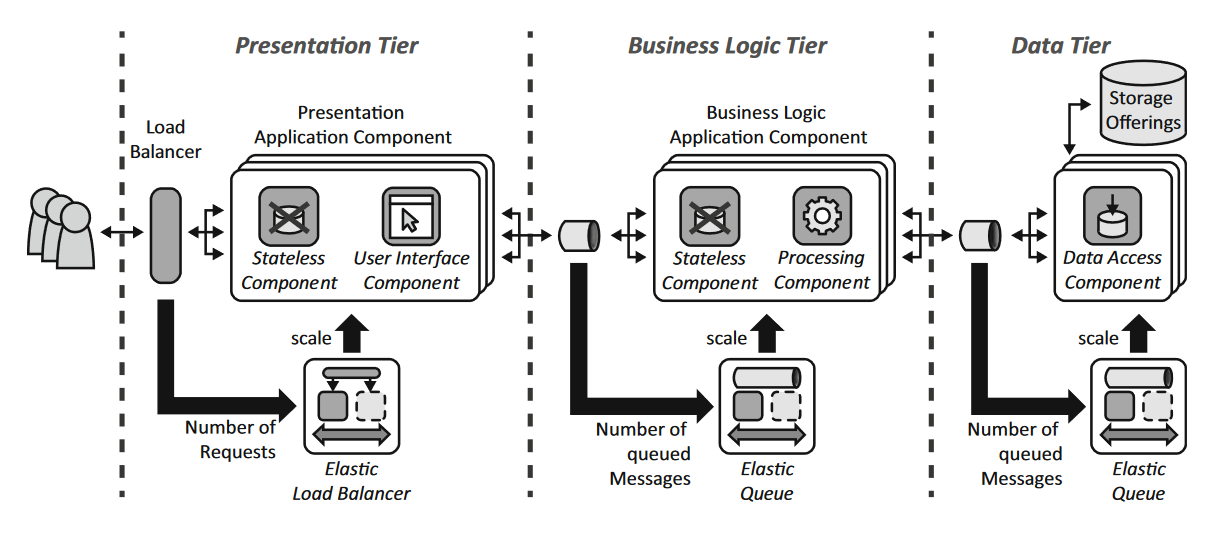
\includegraphics[width=\textwidth]{cloud.PNG}
    \caption{
        Three-tier cloud application\\
        Source: Cloud Computing Patterns
    }
\end{figure}

An additional tier is then added between the user and the application to act as a CDN, to relief some load from the system and improve performances in serving static contents. Overall,
 the resulting application will have five tiers.
The presentation tier will be distributed between the user's device, the CDN and the first server tier of the backend, which will act as a web server. The application tier will map on the second server tier of the backend, while the data tier will map on the third.


\begin{figure}[H]
    \centering
    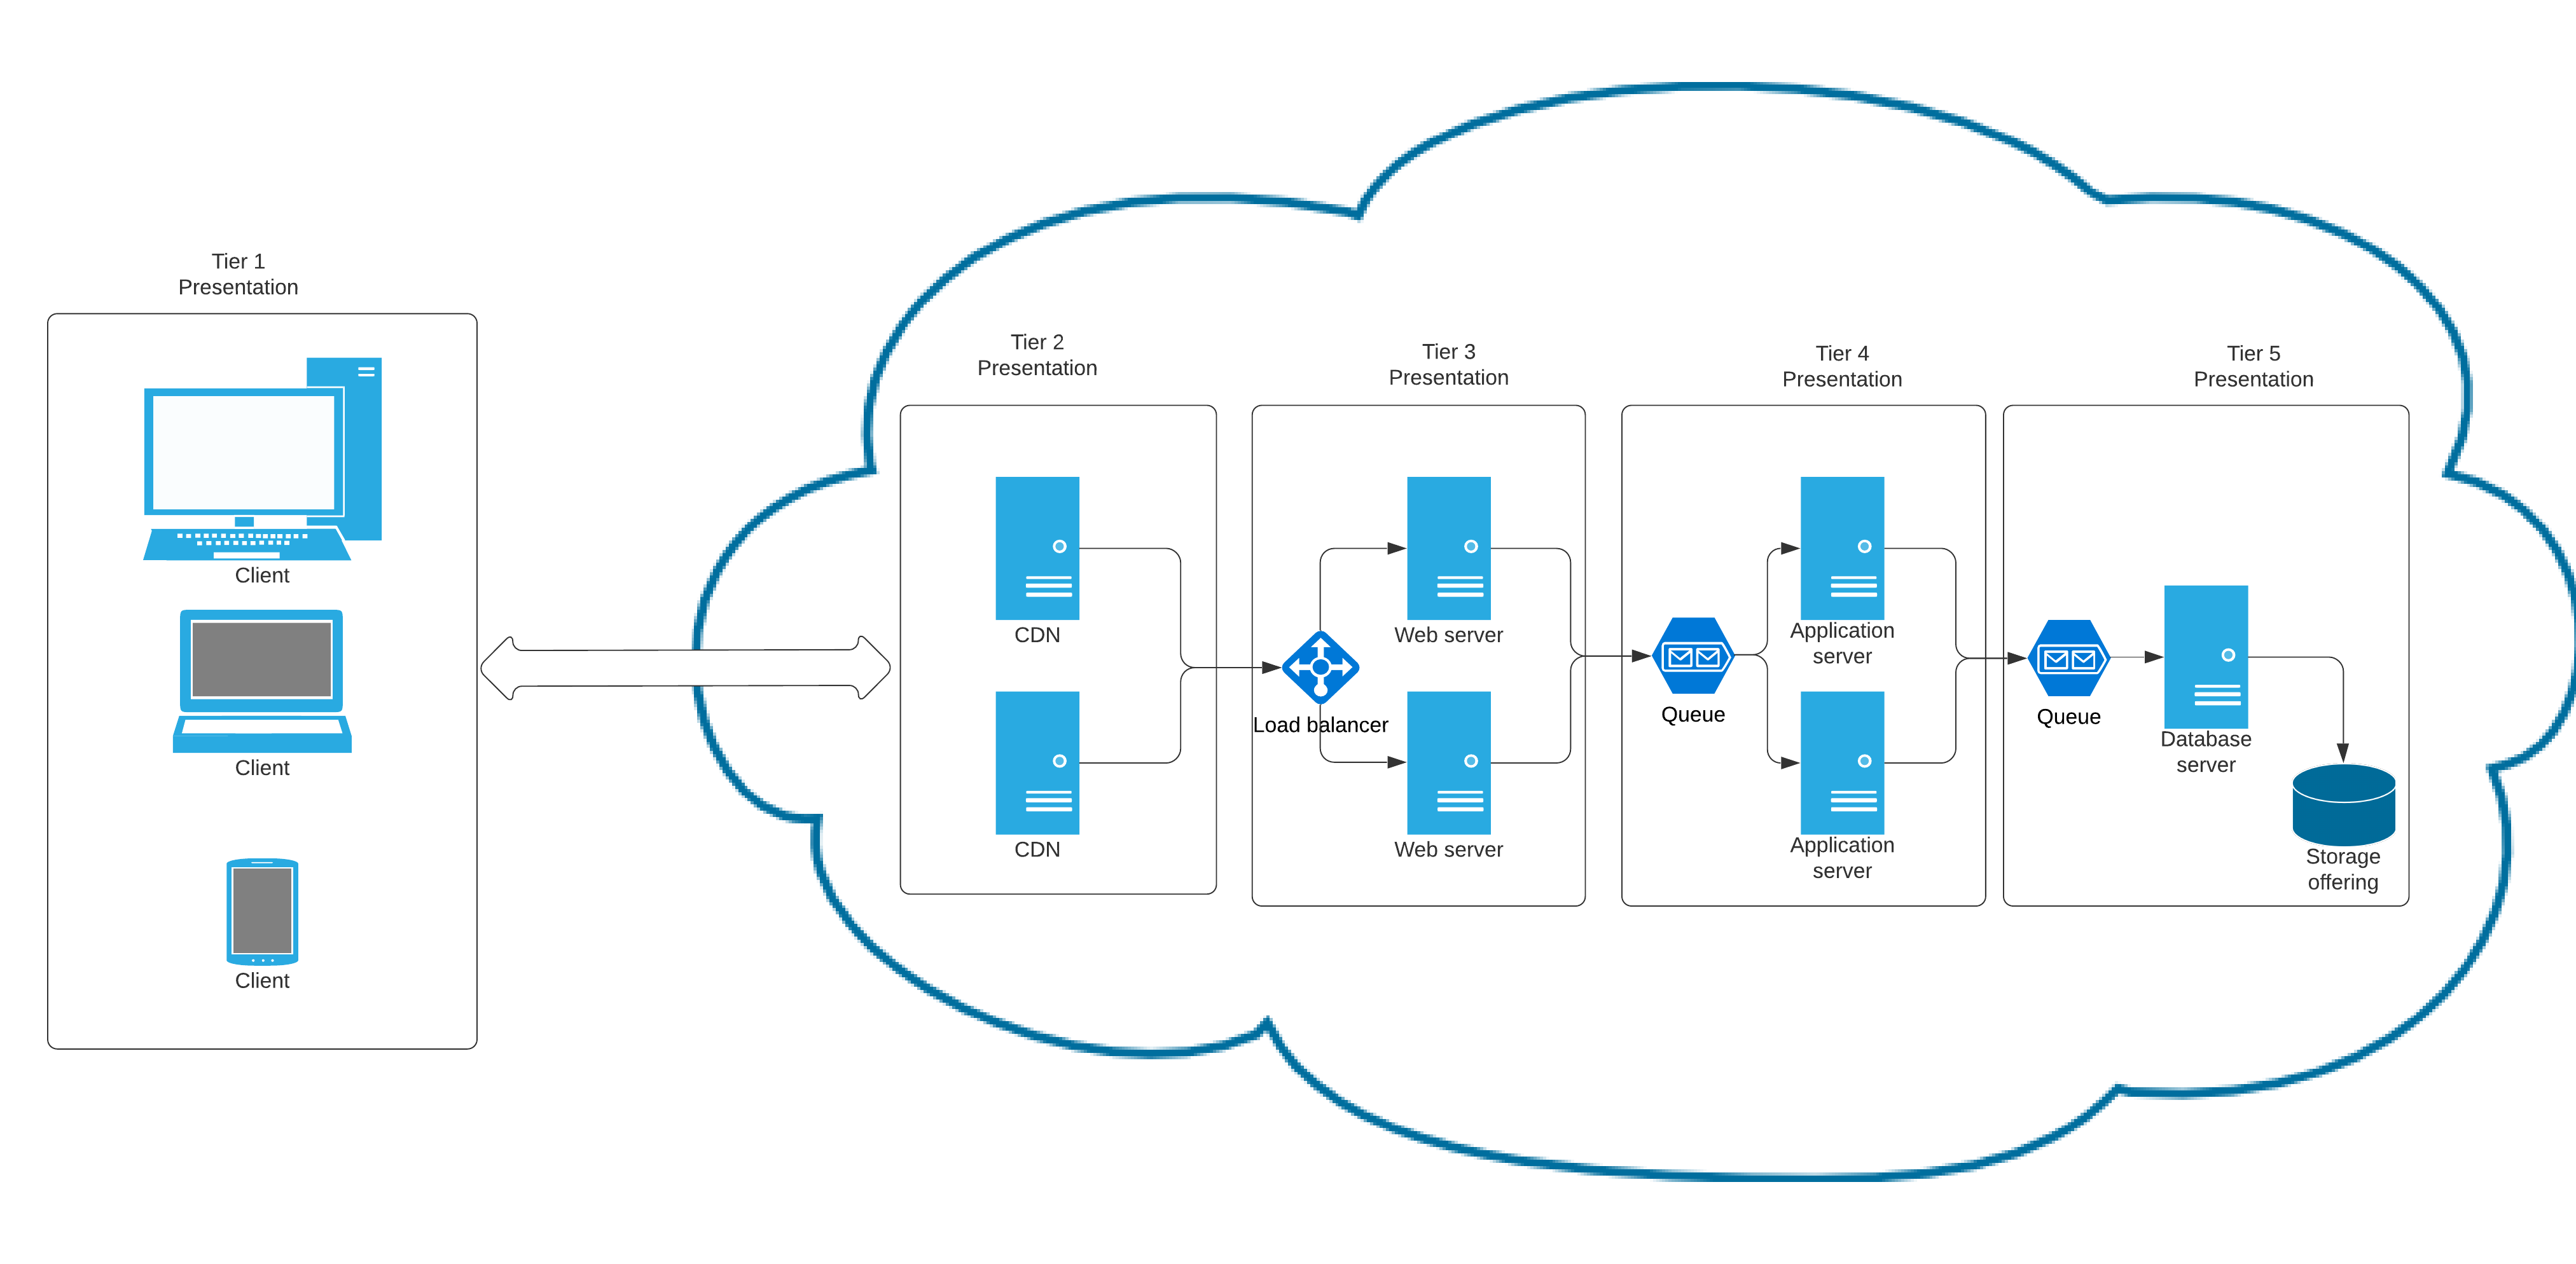
\includegraphics[width=\textwidth]{tiers.png}
    \caption{
        CLup high level architecture
    }
\end{figure}

\end{document}
